\chapter{Apparatus}

SeaQuest is the operational name of Fermilab Experiment \#906 (\emph{E-906}) performed at its Neutrino-Muon (\emph{NM})
experimental area. The experiment was designed
to take \emph{high-intensity beam} at relatively \emph{low center-of-mass energy}, provide
\emph{good mass resolution}, and allow for \emph{accurate target-to-target systematic normalization}.
The apparatus consists of a moving target table, two dipole magnets, 8 hodoscope planes, 24 drift 
chamber planes, and 4 proportional tube planes. Upstream of the target table (towards the beam source),
there is also a Cherenkov counter for beam intensity monitoring and there are
several segmented wire ionization chambers (SWIC's) for beam profiling.

\section{Apparatus Overview}

SeaQuest is a fixed-target experiment. In this style of
experiment, a stationary target is placed in the path of an accelerated beam of particles, as opposed to \emph{collider} 
experiments where two accelerated beams are directed against each other, in opposite directions. The proton beam
interacts with the target material and produces a variety of daughter particles. These daughter particles are 
tracked through a forward spectrometer and selectively filtered dependent on the purpose of the study.

The tuned and monitored 120 GeV proton beam is sent from the Fermilab Main Injector (MI) where the beam
protons strike one of the 7 targets. The high-momentum charged particles that are produced are focused
onto the various detectors with the solid iron dipole magnet, FMAG, or NM3S. 
This solid focusing magnet also sweeps away low-momentum particles and acts as a beam dump / absorber.

\begin{figure}
	\begin{center}
		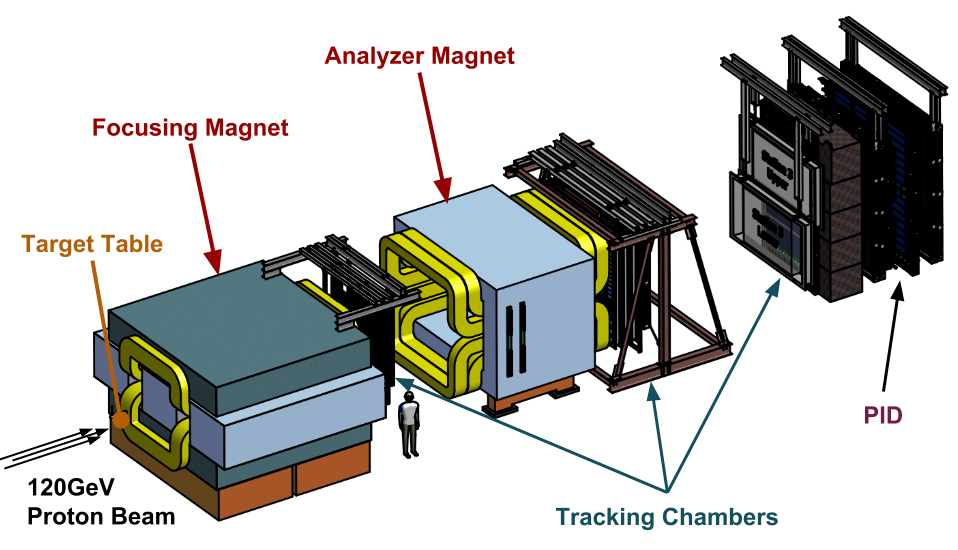
\includegraphics[width=0.75\textwidth]{figures/Spectrometer.png}
		\caption{Perspective view of the SeaQuest spectrometer apparatus.}
		\label{fig:spectrometer-perspective}
	\end{center}
\end{figure}


The SeaQuest Spectrometer (Fig. \ref{fig:spectrometer-perspective}) consists of a focusing magnet to bend charged particles into the experiment's acceptance,
several tracking chambers that record the positions of charged particles through the length of the spectrometer, and
an analyzer magnet to bend the particles between tracking stations. The spectrometer measures particle momenta by
recording the bend of each charged particle as it passed through the analyzer magnet, where the magnetic field is known.
This is performed by reconstructing the trajectory of a particle in one half of the spectrometer (before the
analyzer magnet) and then similarly reconstructing the trajectory of particles in the other half. If two 
trajectories can be matched up, then the particle momentum can be extracted by taking the ratio of the 
magnet's $p_T$-kick to the change in the track's direction.

The spectrometer geometric design and event
triggering selection is optimized to detect oppositely-charged pairs of muons while minimizing the sensitivity
to various sources of unwanted backgrounds. Positive identification of muons is achieved by requiring signals
in the hodoscopes for known muon \emph{``roads''} along with requiring signals in the proportional tubes located at
the farthest end of the experiment, past an iron wall. Electrons and any hadrons are stopped by the solid iron
focusing magnet an iron wall further down, while muons will pass through them unencumbered.

The coordinate system is defined as the following: the \emph{z}-axis points along the beam direction, the
\emph{y}-axis points upwards vertically, and the \emph{x}-axis lies along the horizontal direction
in such a way that a right-handed coordinate system is formed. The terms \emph{upstream} and 
\emph{downstream} are often used when referring directions or regions in the experimental hall.
\emph{Upstream} often refers to the region of the experiment towards the beam source, while
\emph{downstream} refers to everything towards the $+z$ direction. 
The The origin of the coordinate system was chosen to be the point where the proton beam meets 
the \emph{upstream}-facing surface of FMAG, the solid focusing magnet.


\section{Main Injector Proton Beam}

%% January 7th begin

The Fermilab Main Injector (MI) receives protons that have been accelerated by the Radio Frequency Quadrupoles (RFQ), 
the Linear Accelerator (LINAC), and the Booster, and it continues to accelerate them from 8 GeV up to the nomimal energy
of 120 GeV. Along the way, the radio-frequency cavity (RFC) accelerators in the LINAC and the MI ``bunches'' up the
protons such that the beam has its characteristic 53.1 MHz structure. After the period of acceleration, the protons
are then 'scraped off' slowly with each passing \emph{turn} of the collected proton beam and sent down the
Neutrino-Muon (NM) beam delivery line for approximately five seconds of every minute, called a ``slow spill'', or just
``spill''. Beam is extracted using a resonant process, and the extracted beam retains the 53.1 MHz structure of the
Main Injector RFC. Each bunch, or ``bucket'' of protons is less than 2 ns long and the time between bunches is approximately
18.8ns. The spill structure of the beam is depicted in greater detail in Figure \ref{fig:SpillStructure}.

\begin{figure}
	\begin{center}
		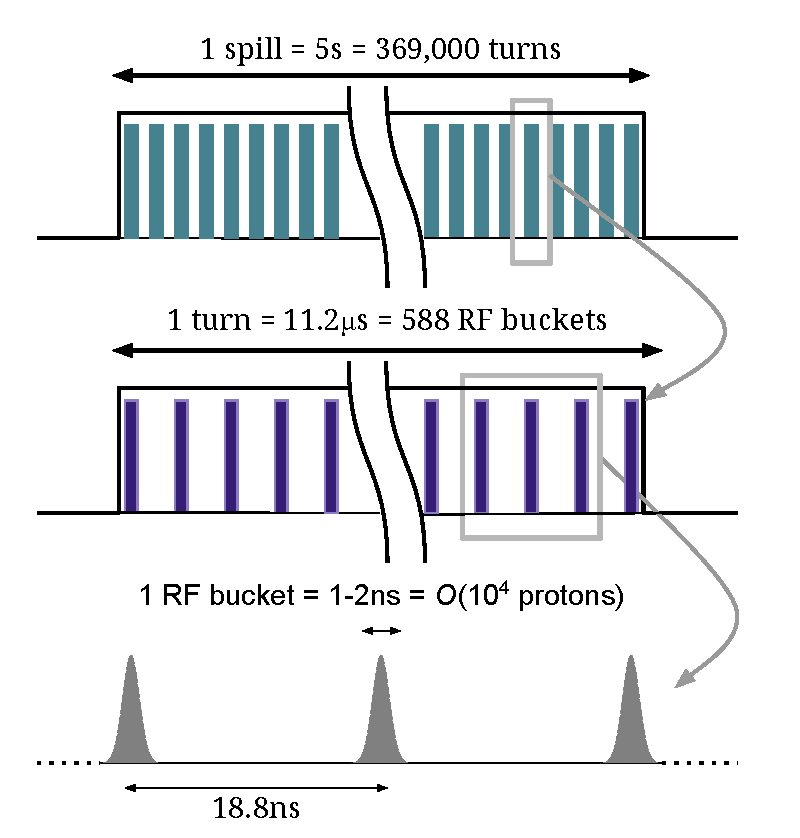
\includegraphics[width=0.55\textwidth]{figures/SpillStructure.pdf}
		\caption{Spill structure of the beam delivered to SeaQuest.}
		\label{fig:SpillStructure}
	\end{center}
\end{figure}

The beam sent to SeaQuest is not uniform in time throughout the spill (in more ways than one).  There are beam bunches in the
MI that are intentionally left empty so that the abort kickers can ramp to full field during a gap in the beam. There are also
bunches left empty to allow the injection kickers to inject 8 GeV protons from the Booster without disturbing bunches of protons
already in the Main Injector.  Typically, 498 of the 588 ``RF buckets'' in the Main Injector contain protons during the SeaQuest
slow spill cycle.  It is the case, however, for SeaQuest, that the intensity of the bunches corresponding to these 498 full
buckets varies greatly throughout the slow spill. On \emph{average}, each bucket will have \emph{O}($10^4$) protons, and the spill
has an intensity of approximately $2\times 10^{12}$ protons per second and therefore about $1\times 10^{13}$ protons delivered per spill.

Several guiding and focusing magnets bend and deliver beam to the NM beamline which serves both the test beam facility and SeaQuest at NM4.
The beam is focused to a width of 250$\mu$m. The profile, position, and intensity are measured along the NM beamline by several detectors.
The intensity of the beam is monitored by an ion chamber (IC) and a secondary emission monitor (SEM) in the NM3 sector. The beam profile
and position are monitored by SWICs and beam-position monitors (BPMs), respectively. The Accelerator Control Network
(ACNET) display of the SWIC readout can be seen in Figure \ref{fig:Profile}. The closest BPMs and SWICs to the spectrometer were
located in NM2 enclosure. The beam profile does not maintain its 250$\mu$m shape, and spreads slightly as it moves towards the
spectrometer. The final beam profile is measured by inspecting the upstream-facing side of the solid targets, and it was found
to be approximately 6mm wide by 1mm high.

\begin{figure}
	\begin{center}
		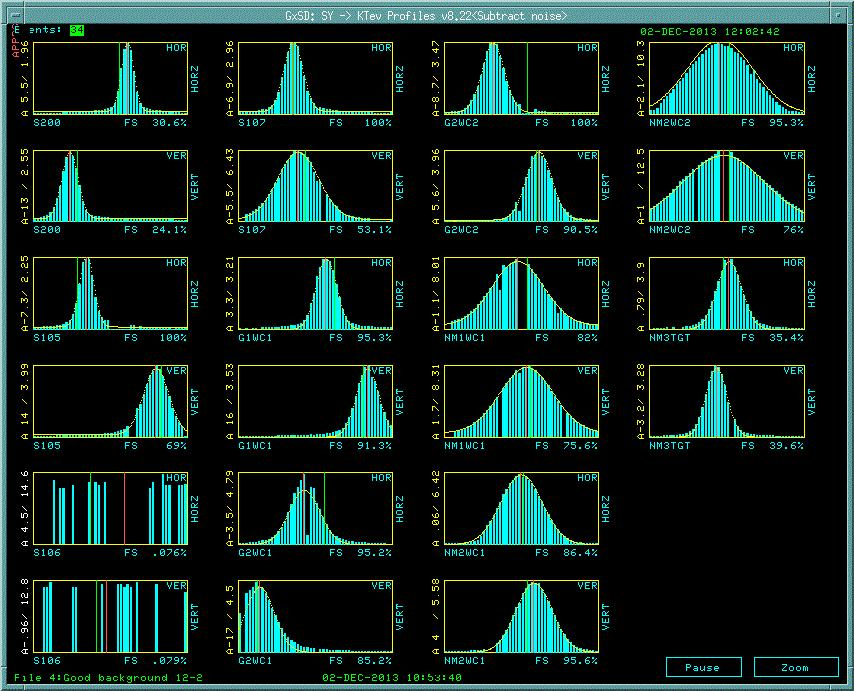
\includegraphics[width=0.65\textwidth]{figures/swic.jpg}
		\caption{Beam profile detailed by SWIC detectors along the NM beam line.}
		\label{fig:Profile}
	\end{center}
\end{figure}

\section{Beam Intensity Monitor}

SeaQuest's trigger system (described in detail later) mostly fires on fake dimuons caused by two low $p_T$ muons from
unrelated pion decays. The hits in downstream hodoscopes from the pions combined with hits in the upstream
hodoscope from two other unrelated particles frequently add up to a false dimuon signal. Since this type of fake
trigger involves four unrelated particles, the probability that a trigger will occur increases with $I^4$, where
$I$ is the intensity of the beam bucket, or the number of protons in the triggered beam bunch.

The SeaQuest data acquisition system (also described later in detail) can read out approximately 3000 events per
second without significant dead time.  During the commissioning run of SeaQuest, the trigger rate was very high and the
trigger dead time was close to 100\%.  These triggers were taken at such high beam intensities that the occupancy
of all SeaQuest detector elements was more than 50$\%$, making pattern recognition essentially impossible
(see Figure. \ref{fig:splat}). The Beam Intensity Monitor (BIM) was designed to solve this problem.

\begin{figure}
	\begin{center}
		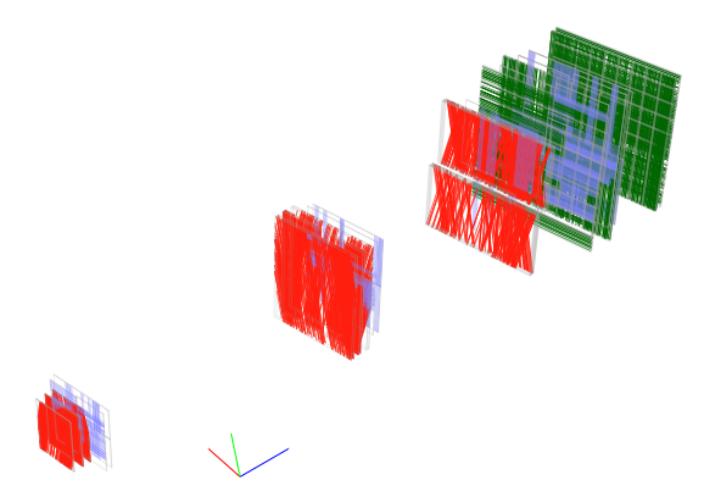
\includegraphics[width=0.5\textwidth]{figures/splat2.png}
		\caption{A single high-intensity event with majority of all detector elements firing off. White space within the rectangles indicates inactive elements whereas red, blue, and green represent elements which have fired during that event. Track reconstruction in these cases is impossible.}
		\label{fig:splat}
	\end{center}
\end{figure}

The SeaQuest Beam Intensity Monitor (BIM) senses when the beam intensity is above a programmable threshold.
If an RF bucket with an intensity above this threshold is detected, the BIM sends a signal to inhibit
certain triggers until the intensity once more falls below the threshold. The inhibit threshold is tuned
frequently as trigger and beam conditions change, but the inhibit threshold is typically set at approximately
95,000 protons per RF bunch. For reference, a full RF bucket at an intensity of $2\times 10^{12}$ protons per
spill is $\approx$10,000 protons.

The beam intensity is measured using an atmospheric pressure gas Cerenkov counter. A gas mixture of 80$\%$ Argon and 20$\%$ CO$_2$
is used as the Cerenkov radiator. The counter and readout electronics were designed to have $O(ns)$ time resolution, and a linear
response over a large dynamic range.  A diagram of the counter is shown in Figure~\ref{fig:BIMCerenkov}.  A 45 degree aluminized
Kapton mirror directs light to a single photomultiplier tube.  A \emph{baffle} of black construction paper held parallel to the
mirror ensures that the proton path length through the light-radiating gas with respect to the mirror is independent of beam
position. A two-inch diameter 8-stage photomultiplier tube (PMT) is positioned close to the mirror so that all Cerenkov light created between the baffle and the mirror falls directly on the aperture of the PMT. It was observed during the commissioning run
that after exposure to $\approx 3 \times 10^{17}$ protons (~3 weeks of uninterrupted usage), the mirror reflectivity is significantly reduced in the beam spot, and the mirror then needs to be replaced.

\begin{figure}
	\begin{center}
		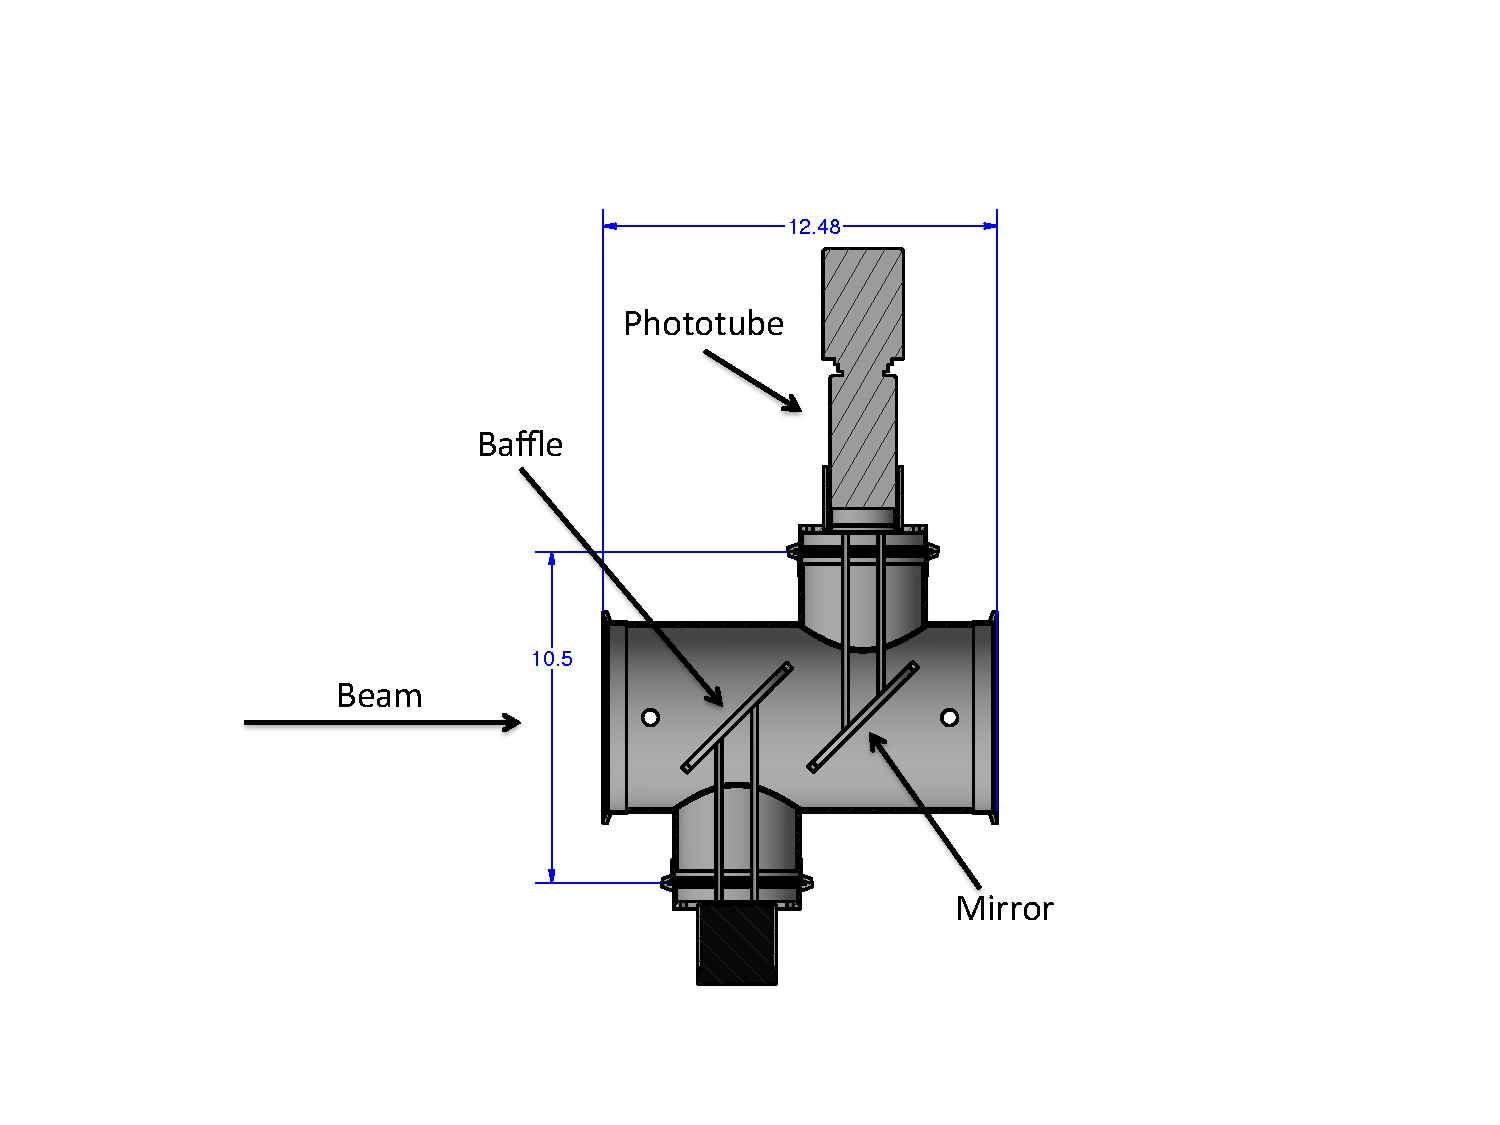
\includegraphics[width=0.6\textwidth]{figures/BIMCerenkov.pdf}
		\caption{The Beam Intensity Monitor (BIM) Cerenkov counter. Measurements are in inches.}
		\label{fig:BIMCerenkov}
	\end{center}
\end{figure}

The signal from the BIM is integrated and digitized using a custom charge (Q) integrator and encoder (\emph{QIE}) integrated circuit board, which comes from a family of circuits used first by the KTeV experiment at Fermilab\cite{QIE}. The chip is clocked with the Main Injector RF clock and provides an ADC (analog-digital conversion) every 18.8ns clock cycle. The light incident on
the photomultiplier tube is attenuated using neutral density filters (NDF's) so that the QIE least count corresponds to
$\sim$30 protons per beam bunch.

In addition to inhibiting triggers during high-intensity periods of beam, the BIM readout module also provides critical
information used to calculate the number of protons incident on the SeaQuest targets while the experiment is ready
and able to trigger. This value is needed to normalize SeaQuest cross section measurements. The BIM readout module provides the following:
\begin{itemize}
\item Sum of all ADC signals for the entire spill (QIESum).
\item Sum while inhibit is asserted at trigger logic.
\item Sum during trigger dead time.
\item A snapshot of beam intensity 16 buckets before and after the triggered RF bucket
\end{itemize}

These are used to calculate a ratio of protons that were `live' (the experiment can trigger) via the following:
\begin{eqnarray}
	liveRatio & = & \frac{QIESum - (inhibit\ sum + dead\ time\ sum)}{QIESum} \\
	liveProton & = & totalProton \cdot liveRatio
	\label{eqn:liveproton}
\end{eqnarray}
where ``totalProton'' is the intensity value recorded from the SEM detector located just upstream of the BIM Cerenkov counter.
The SEM itself is calibrated by foil activation. The snapshot of the triggered RF bucket intensity along with the 32
surrounding RF bucket intensities is used for studies and corrections of the rate-dependent effects on detector efficiencies
and reconstructed measurements.

\section{The SeaQuest Targets}

\begin{table}[p]
	\begin{center}
		\begin{tabular}{c c c c c c c}
			\parbox{1.5cm}{\centering{~\\Position} } & \parbox{1.5cm}{\centering{~\\Material} }  &\parbox{1.5cm}{\centering{Density\\{[g/cm$^3$]}} }  &  \parbox{1.75cm}{\centering{Thickness\\{[cm]}} }& \parbox{2cm}{\centering{Interaction\\Length} }&  \parbox{1.5cm}{\centering{Spills/\\Cycle\\(\%spills)} } \\ [0.5ex] \hline
			1 & $H_2$     & 0.07065 & 50.8  & 0.06902 & 10 (43\%) & \\
			2 & Empty     & NA      & NA    & 0.0016  & 2 (9\%)  & \\
			3 & $D_2$     & 0.1617  & 50.8  & 0.1144  & 5 (22\%)  & \\
			4 & None      & NA      & NA    & 0.0     & 2 (9\%)  & \\
			5 & Iron      & 7.874   & 1.905 & 0.1135  & 1 (4\%)  & \\
			6 & Carbon    & 1.802   & 3.322 & 0.0697  & 2 (9\%)  & \\
			7 & Tungsten  & 19.30   & 0.953 & 0.0958  & 1 (4\%)  & \\ [0.5ex] \hline
		\end{tabular}
		\caption{Characteristics of the seven SeaQuest target positions.  The ``Spills/Cycle'' is only a typical configuration and can vary according to needs and running configurations.  The non-zero interaction length of the empty flask is due to the 51$\mu$m-thick stainless steel end-caps of the flask and the 140 $\mu$m-thick titanium windows of the vacuum vessel that contains it.}
		\label{tab:target-materials}
		
	\end{center}
\end{table}

\begin{figure}[p]
	\begin{center}
		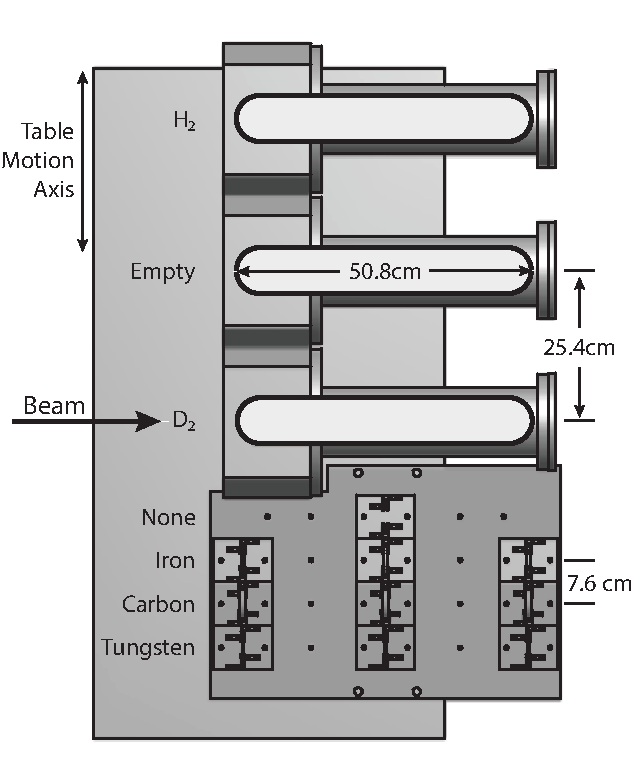
\includegraphics[width=0.65\textwidth]{figures/target-tableLayout.pdf}
		\caption{The layout of the target table and its seven target positions, as seen from above.}
		\label{fig:table-layout}
	\end{center}
\end{figure}


A wide range of atomic weights (from 2 to 184) is required to do an A-dependence study of the Drell-Yan process.
At SeaQuest, the targets used are $^1H (\ell),\ ^2H (\ell),\ C,\ Fe,\ $and$\ W$. In addition to the two liquid targets
and the three solid targets, two positions on the target table were used for measuring background signal rates:
an empty flask, identical to the flasks used for the $^1H$ and $^2H$ targets, and a single empty solid target holder.
Colloquially speaking: the $^1H$ target is interchangeably referred to as the liquid hydrogen target, $\ell H_2$,
\emph{LH2}, or $H_2$; $^2H$ is likewise referred to as the liquid deuterium target, $\ell D_2$, \emph{LD2}, or $D_2$;
the empty flask is referred to as the ``Empty'' target; the empty solid target holder is referred to as the ``None'' target.

These are all mounted on a laterally-moving, remotely positionable table (in the $\pm x$ direction), able to move
over a range of 91.4cm. The table's center is located at $(0, 0, -1.25)$ meters, directly in front of the upstream face
of FMAG, the solid iron focusing magnet. Because of the $\sim$5.0cm diameter of the targets and the 6x1mm dimensions of the beam, the targeting efficiency was 100\%. The details of the target materials are summarized in Table \ref{tab:target-materials}, and the layout of the target table can be seen in \ref{fig:table-layout}.

The $H_2$ gas used is ``Ultra High Purity 5.0 Grade'' or 99.999\% pure.  The deuterium has come from two different
sources.  The first of these is Fermilab-provided supply of gas left over from previous bubble chamber experiments.
This gas was known to have a small hydrogen contamination and was measured by mass spectroscopy to have a composition
of 85.2\% D$_2$, 12.7\% HD, 1.2\% $^4$He, and 0.8\% H$_2$ by mole. As analysis of experimental data commenced, 
handling the ramifications of the D$_2$ impurity came under focus. Unexpected bottle-to-bottle variation in contamination
became evident, and the sample-taking methodology itself for spectroscopy became suspect of introducing contamination.
In order to no simplify analysis and reduce the substantial complexity and cost of further gas analysis, SeaQuest switched
to commercially available ``Research Grade'' D$_2$, which is better than 99.6\% pure with virtually all HD to balance.
The data analyzed in this paper deals with the impure D$_2$ target material before this switch. Further information on
the D$_2$ composition and how it is handled in analysis will be covered in Chapter 4.

%10'' apart to approximate the 20'' 
%  more closely spaced (6.73'').

Each of the three solid target positions is divided into three disks of 1/3 the total thickness provided in Table \ref{tab:target-materials}. These disks are spaced 25.4cm apart to approximate the distribution of the liquid target, thereby minimizing target-dependent variation in spectrometer acceptance. The one exception to this is that during the Run II period the iron plugs were more closely spaced (17.1cm). The decision to place these
iron disks closer together than the rest during Run II is still unclear.

The target table is able to move between two different targets in about 30 seconds. This allows a change in target in the 55 seconds between successive spills. With this frequent target interchange, the systematic uncertainties associated with drifts in beam characteristics, monitor gains, and detector efficiencies are reduced to a minimum when investigating A-dependent ratios. How much beam time each target received is determined by interaction lengths of the targets along with the amount of statistics desired for certain targets. As the flagship measurement of SeaQuest is the $\bar{d}/\bar{u}$ asymmetry, more emphasis was placed on the hydrogen and deuterium than the nuclear targets. The spills per cycle and beam time allocation can be found in Table \ref{tab:target-materials}.

\section{Focusing and Analyzing Magnets}

Two large dipole magnets are used in the experiment to be select forward going ($x_F > 0$) dimuons, reject low-momentum particles, and analyze their kinematic characteristics. The most upstream magnet, denoted ``FMAG'', is a solid iron A-frame magnet with an aperture of 1.22m in the $x$-direction and 66cm in the $y$-direction. It is assembled from 43.2cm x 160cm x 503cm iron slabs, as shown in Fig.~\ref{fig:FMag}. The magnet has no air gap, and the iron has extremely high purity, allowing a 2000A excitation current to generate a nearly constant, central magnetic field of 1.9 Tesla (yielding a 2.91 GeV/c total magnetic deflection). The field is generated by exciting the embedded aluminum \emph{``bedstead''} coil to 2000 Amps at 25 Volts (50 kW).  The current exciting FMAG is monitored by the Fermilab ACNET system and is broadcast to the SeaQuest slow data acquisition system every acceleration cycle. The excitation is also input to the beam-disabling safety system in order to prevent beam from hitting the SeaQuest spectrometer when FMAG is not fully powered. FMAG also acts as the beam dump for the 120 GeV beam. There is a 5cm diameter by 25cm deep bore drilled into the upstream end of FMAG (recall, this is the origin of the experiment's coordinate system).  The 120 GeV protons that do not interact in the SeaQuest targets 125cm upstream of FMag, interact in the central iron slab.  Most of the 2.0 kW beam power is dissipated in this slab and is eventually conducted to the coils and external surfaces to be radiated away.

\begin{figure}
	\centering
	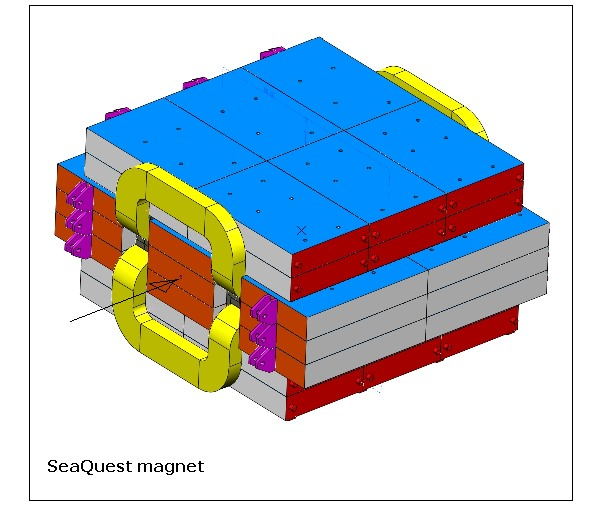
\includegraphics[width=8cm]{figures/FMAG}
	\caption{Perspective drawing of FMAG's aluminum coils embedded in an arrangement of iron slabs.}
	\label{fig:FMag}
\end{figure}

The downstream magnet, denoted ``KMAG'', is a 300cm long iron rectangular magnet with a 289cm wide by 203cm high central air gap.  It was originally constructed by the KTeV collaboration~\cite{PhysRevD.67.012005} at Fermilab.  It is excited to a central field of 0.4 Tesla (0.402 GeV/c magnetic deflection) by 1600 Amps at 270 Volts (430kW).  The spatial distribution of the magnetic field in KMAG was measured by the KTeV group and re-verified by SeaQuest.  In normal running conditions, both FMag and KMAG bend muons horizontally in the same direction. This two-magnet configuration is often referred to as a focusing spectrometer.

The 2.91 GeV/c and 0.402 GeV/c magnetic deflection delivers a transverse-momentum ($p_T$) kick along the to charged particles passing through the spectrometer. The magnets bend the paths of the muon in the $\pm x$ direction, with the sign depending on the orientation of the magnetic fields and the particles' charges. Between Run II and Run III of data taking, the current direction was reversed, thereby reversing the direction of the magnetic fields. During Run II, the magnetic fields were pointing in the $-y$ direction, and in Run III, the magnetic fields were flipped to point in the $+y$ direction. This was done for two reasons: (1) to identify any left-right asymmetries in the experiment, and (2) to limit the amount of radiation on the electronics in the experimental hall, as the large amount of positive particles were being swept directly towards the electronics racks during Run II.

\section{Beam Dump, Shields, and Absorbers}

In order to prevent damage to the downstream detectors from the beam and reduce signals from incidental radiation, the spectrometer is designed with a beam dump and two hadron absorber walls. Approximately 125cm downstream of the target table
is the water-cooled beam dump whose upstream face is located at $(0.0, 0.0, 0.0)$ m. The beam dump is one of the many solid iron 5m blocks that fill and surround the FMAG coils. The whole length of the beam dump along the beam axis is equivalent to $\approx 35$ nuclear interaction lengths of iron. 

Between the downstream face of FMAG and Station 1, there is a 2 cm thick wall of borated polyethylene which is put in place as a fast neutron shield. This material is 5\% boron by weight, with the rest being polyethylene. The polyethylene contains high hydrogen content, making it an effective fast neutron radiation shield, slowing down the fast neutrons down to thermal speeds. The boron in the material provides attenuation of thermal neutrons, thus reducing the levels of capture-gamma radiation elsewhere in the experiment. Borated polyethylene at this thickness is a common and optimal neutron shielding material for areas of low to intermediate neutron flux where the temperature is below $82^\circ$C \CN. These conditions make the downstream side of FMAG ideal for its placement.

Farther downstream, there is another hadron absorber wall located between Station 3 and Station 4. The absorber wall consists of a stack ot 98cm thick iron blocks. This is an equivalent of $\approx 6$ nuclear interaction lengths. The purpose of this wall is to identify muons at the rear of the apparatus by effectively blocking all other types of particles. The only charged particles which can penetrate this absorber wall are muons.

\section{Tracking Detectors}

The tracking detectors are the instruments used for measuring the values of the kinematic variables of the dimuon pairs. Several different types of detectors are grouped together to form a detector \emph{Station}. The types of detectors used are hodoscopes, wire chambers, and proportional tubes. There are four stations throughout the experimental hall that provide tracking information at different points along the spectrometer, numbered from 1 to 4 in order of increasing $z$. Station 1 is located between FMAG and KMAG. Station 2 is located at the downstream face of KMAG. Station 3 and 4 are just upstream and downstream, respectively, of the iron absorber wall. The Station layout can be seen in Fig. \ref{fig:stations}

\begin{figure}
	\centering
	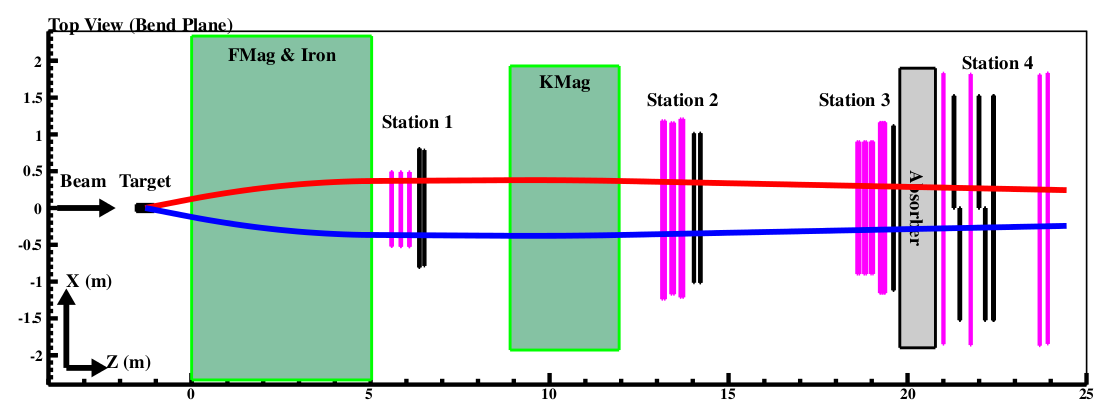
\includegraphics[width=0.75\textwidth]{figures/stations.png}
	\caption{Spectrometer layout of FMAG, KMAG, and Detector Stations 1-4.}
	\label{fig:stations}
\end{figure}

\subsection{Triggering Hodoscopes}

Hodoscope arrays are located at each of the four detector stations. These detectors' primary usage is to select events with two opposite-signed muon tracks in them. Certain `roads' through the spectrometer are defined in the fast trigger logic, and when two desired roads are observed in a given event, the trigger system tells the data acquisition systems to record that event's data. In addition to this, the hodoscopes provide analysts with the ability to discard or ignore certain hits in adjacent chambers for which there is no corresponding nearby hodoscope hit. This is useful in decreasing the hit multiplicities in the wire chambers, which in turn decreases the combinatoric complexity of reconstruction algorithms.

Each of the eight hodoscope planes are split into two halves: top and bottom in the case of planes with vertically-oriented paddles, or left and right for planes with horizontally-oriented paddles (denoted by `T', `B', `L', and `R', respectively). In each half-plane, the hodoscopes are a set of long rectangles arranged `picket fence'-style with a small 0.3175cm overlap, as to prevent any particles from possibly slipping between paddles. A single hodoscope detector element is composed of plastic scintillator material connected to Philips XP 2008 photomultiplier tubes (PMT) by plexiglass light guides. Stations 1, 2, and 4 each have two hodoscope planes, with planes of both vertically- and horizontally-oriented paddles (for measuring in $x$ and $y$, respectively). Station 3 only has vertically-oriented plane, and thus measures in the $x-$direction only, which is in the experiment's $x-z$ bend plane. The hodoscope planes are named according to detector station and the direction that they measure. For example, the $y$-measuring hodoscope plane in Station 2 is called ``H2Y''. The individual half-planes are named according to detector station and which half it is of the two. For example, the top half of the $x$-measuring hodoscope plane in Station 1 is referred to as ``H1T''. As such, the ``H3X'' detector is composed of ``H3T'' and ``H3B''. The detailed specifications of each hodoscope plane are given in Table \ref{tab:hodoscopes}. A precise alignment of the hodoscopes was achieved by examining the distributions of positions of tracked muons at each hodoscope plane when a given hodoscope element in that plane was fired.

\begin{table}[bthp]\centering
  \begin{tabular}{llllll}
    \hline
    \hline
    Detector & Paddle & Overlap & \# of paddles & Width $\times$ Height & $z$-position [cm] \\
    & Width & [cm] & (per half-plane) & (per half-plane) &  \\
    & [cm] & & & [cm] $\times$ [cm] & \\
    \hline
    H1X & 7.32 & 0.3175 & 23 & 162 $\times$ 70 & 666 \\
    H1Y & 7.32 & 0.3175 & 20 & 79 $\times$ 140 & 653 \\
    H2X & 13.00 & 0.3175 & 16 & 203 $\times$ 152 & 1421 \\
    H2Y & 13.00 & 0.3175 & 19  & 132 $\times$ 241 & 1400 (L), 1406 (R) \\
    H3X & 14.59 & 0.3175 & 16  & 228 $\times$ 168 & 1959 \\
    H4X & 19.65 & 0.3175 & 16  &  305 $\times$ 183 & 2234 (T), 2251 (B) \\
    H4Y1 & 23.48 & 0.3175 & 16  & 152 $\times$ 366 & 2130 (L), 2146 (R) \\
    H4Y2 & 23.48 & 0.3175 & 16  & 152 $\times$ 366 & 2200 (L), 2217 (R)\\
    \hline
    \hline
  \end{tabular}
  \caption{Parameters of all hodoscope planes. $z$-positions of H2Y and H4 half-planes are offset slightly due to the half-planes themselves overlapping.}
  \label{tab:hodoscopes}
\end{table}

\subsection{Drift Chambers}

Each of Stations 1, 2 and 3 is equipped with a drift chamber (DC) to measure the passing $x$ and $y$ positions of muons at its $z$ location, with each DC flat vertical to the $z$ axis, and a drift cell is of the box shape.. These measured positions are critical for reconstructing the trajectory of muons, and thereby their kinematics. Each DC contains six drift chamber planes, arranged in three pairs with parallel wire orientations (each pair referred to as a ``view''). Wires oriented vertically ($x$-measuring) are referred to as being in the ``X'' view, and at angles of $+14^\circ$ and $-14^\circ$ with respect to the $y$-axis are the ``V'' and ``U'' planes, respectively. The second plane in each view is offset from the first by one half of a wire-to-wire distance (\emph{``cell width''}) in order to resolve the left-right ambiguity of drift direction. This offset plane of each pair is referred to as the \emph{primed} plane, and is denoted with a `$\prime$'. So, in each DC, there are X, X$^\prime$, U, U$^\prime$, V, and V$^\prime$ planes, with primed and unprimed planes (like X and X$^\prime$) constituting a view.

The individual drift chambers at Stations 1 and 2 are called ``D1'' and ``D2'', respectively. Station 3 has two drift chambers, since the desired acceptance area it has to cover is substantially larger than one DC can cover. These are split vertically to cover the top and bottom halves, and are called ``D3p'' and ``D3m'' where ``p'' and ``m'' stand for ``plus'' and ``minus''. Table~\ref{table:cham:param} summarizes the parameters of the DC's. D1 and D3m have been upgraded during the data taking, as listed in Tab.~\ref{tab:cham:comb1}. This original and upgraded versions are referred to as D$N$.1 and D$N$.2, respectively.

\begin{table}[bthp]\centering
  \begin{tabular}{cc|cccc}
    \hline \hline
    Chamber & Plane & Number   & Cell  & Width            & $z$-position \\
            &       & of wires & width & $\times$ height  &      \\ 
            &       &          & [cm]  & [cm] $\times$ [cm] & [cm] \\ 
    \hline
    D1.1    & X     & 160      & 0.64  & 102 $\times$ 122 &  617    \\
             & U, V  & 201      & 0.64  & 101 $\times$ 122 & $\pm$20 \\
    D1.2    & X     & 320      & 0.50  & 153 $\times$ 137 &  617    \\
             & U, V  & 384      & 0.50  & 153 $\times$ 137 & $\pm$1.2 \\
    D2      & X     & 112      & 2.1   & 233 $\times$ 264 & 1347    \\
             & U, V  & 128      & 2.0   & 233 $\times$ 264 & $\pm$25 \\
    D3p     & X     & 116      & 2.0   & 232 $\times$ 166 & 1931    \\
             & U, V  & 134      & 2.0   & 268 $\times$ 166 & $\pm$6  \\
    D3m.1   & X     & 176      & 1.0   & 179 $\times$ 168 & 1879    \\
             & U, V  & 208      & 1.0   & 171 $\times$ 163 & $\pm$19 \\
    D3m.2   & X     & 116      & 2.0   & 232 $\times$ 166 & 1895    \\
             & U, V  & 134      & 2.0   & 268 $\times$ 166 & $\pm$6  \\
    \hline
    \hline
  \end{tabular}
  \caption{Parameters of all chambers.
  	Those of primed planes are almost the same as of unprimed planes.
  	The $z$-positions of U and V planes are relative to those of X planes.
  }
  \label{table:cham:param}
\end{table}

\begin{table}[bthp]\centering
  \begin{tabular}{ccc}
    \hline
    Run & Period & Chamber combination \\
    \hline
    1 & 2012 Mar.-2012 Apr.  &  D1.1, D3m.1 \\
    2 & 2013 Nov.-2014 Aug.  &  D1.1, D3m.2 \\
    3 & 2014 Nov.-2015 May   &  D1.1, D3m.2 \\
    3 & 2015 Jun.-2015 Jul.  &  D1.2, D3m.2 \\
    4 & 2015 Sep.-   &  D1.2, D3m.2 \\
    \hline
  \end{tabular}
  \caption{Combination of D1 and D3m chambers per data taking period.}
  \label{tab:cham:comb1}
\end{table}

The acceptance size of each chamber has been adjusted with a Drell-Yan event simulation in order to be as sensitive as possible to the $x_2$ range of interest. Particularly, the greater the acceptance width is, the higher the reach in $x_2$ is. This makes the hit-rate tolerance of the chambers a key feature, because the spectrometer is exposed to a large number of background particles, particularly near the edges where the desired $x_2$ events occur. It is particularly significant for the most-upstream station (i.e.~Station 1) which receives the highest hit rates. Experimental data shows that the rate tolerances are 3.0 MHz/wire at D1, 1.6 MHz/wire at D2 and 0.7 MHz/wire at D3 with a beam intensity of $5\times 10^{12}$ protons/spill. The gas-amplification gain should not be degraded under these hit rates.

For Run 2 and beyond, the gas mixture used for almost all the chambers is Argon:Methane:CF4 (88\%:8\%:4\%) with a drift velocity of about 20 $\mu$m/ns. A ``fast gas'' mixture used for D1.2 (upgraded D1) is Argon:CF4:Isobutane:Methylal (68\%:16\%:13\%:3\%) with a drift velocity of 50 $\mu$m/ns and thereby a better hit-rate tolerance. This is ``fast'' in comparison to the $\approx 20\mu$m/ns rest of the DCs. The spatial resolution of each plane is required to be 400$\mu$m, which corresponds to a momentum resolution of $\Delta p / p = 0.03 \cdot p$ (GeV/$c$). The resolution of dimuon invariant mass is dominated by the multiple scattering in FMAG; the chamber momentum resolution is about 10\% of the total mass resolution at maximum.

The D1.1, D2 and D3m.1 chambers have been inherited from previous Drell-Yan experiments that have been conducted at Fermilab.
Chambers D2 and D3m.1 have their origin in E-906~\cite{PhysRevD.43.2815} and D1.1 is from SeaQuest's direct predecessor, E-866/NuSea~\cite{PhysRevLett.80.3715, Towell:2001nh}. Since these chambers haven't been used for decades after the previous experiment, they had to be refurbished by restringing $\approx 30\%$ of their sense wires due to them being loose or broken. Newly supplied electronic readout boards were also mounted on these chambers.

The D3p and D3m.2 chambers were designed and constructed specifically for this experiment in order to cover the large acceptance required at Station 3. D3p was newly constructed by the TokyoTech SeaQuest collaborators and was shipped from Japan to Fermilab. The first part of data taking, Run 1, was carried out using D3m.1 while preparing for the construction of D3m.2. The newer D3m.2 is wider than D3m.1 by 25 cm at each side, allowing the high-$x_2$ statistics on $\bar{d}/\bar{u}$ and $Y_A / Y_{^2H}$ to increase by $\approx 20\%$ at $x_2 \sim 0.3$ and $\approx 10\%$ at $x_2 \sim 0.4$. The operational stability also improved, as D3m.1 suffered from frequent dead/noisy wires, HV trips, and leak currents. The D1.2 chamber was also designed and constructed for this experiment by the University of Colorado Boulder. As it is wider than D1.1 by 25 cm at each side and greater hit-rate tolerance, the anticipated statistics is expected in the high-$x_2$ region is expected to increase still more. It was installed in the experimental hall near the end of Run 3.

\subsection{Proportional Tubes}

Downstream of Station 3 and the 1 m thick iron hadron absorber wall is Station 4 with its hodoscope planes and proportional tube  detectors (prop tubes). At Station 4, the only beam-induced particles that remain that can leave tracks in an ionization detector are high energy muons. The prop tubes enable the task of muon particle identification (PID) for the experiment, and consist of four planes. Each detector plane is made of 9 prop-tube modules, with each module assembled from 16 12-ft long 2" diameter prop-tubes staggered to form two sub-layers. The first and fourth planes are oriented along the horizontal direction (tubes parallel to the floor) to provide positional measurements in $y$, as shown in Fig.~\ref{fig:proptube:xzview}. The second and third planes are arranged vertiacally to measure $x$-position as shown in and Fig.~\ref{fig:proptube:yzview}.

\begin{figure}
	\centering
	\begin{minipage}[t]{0.49\linewidth}
		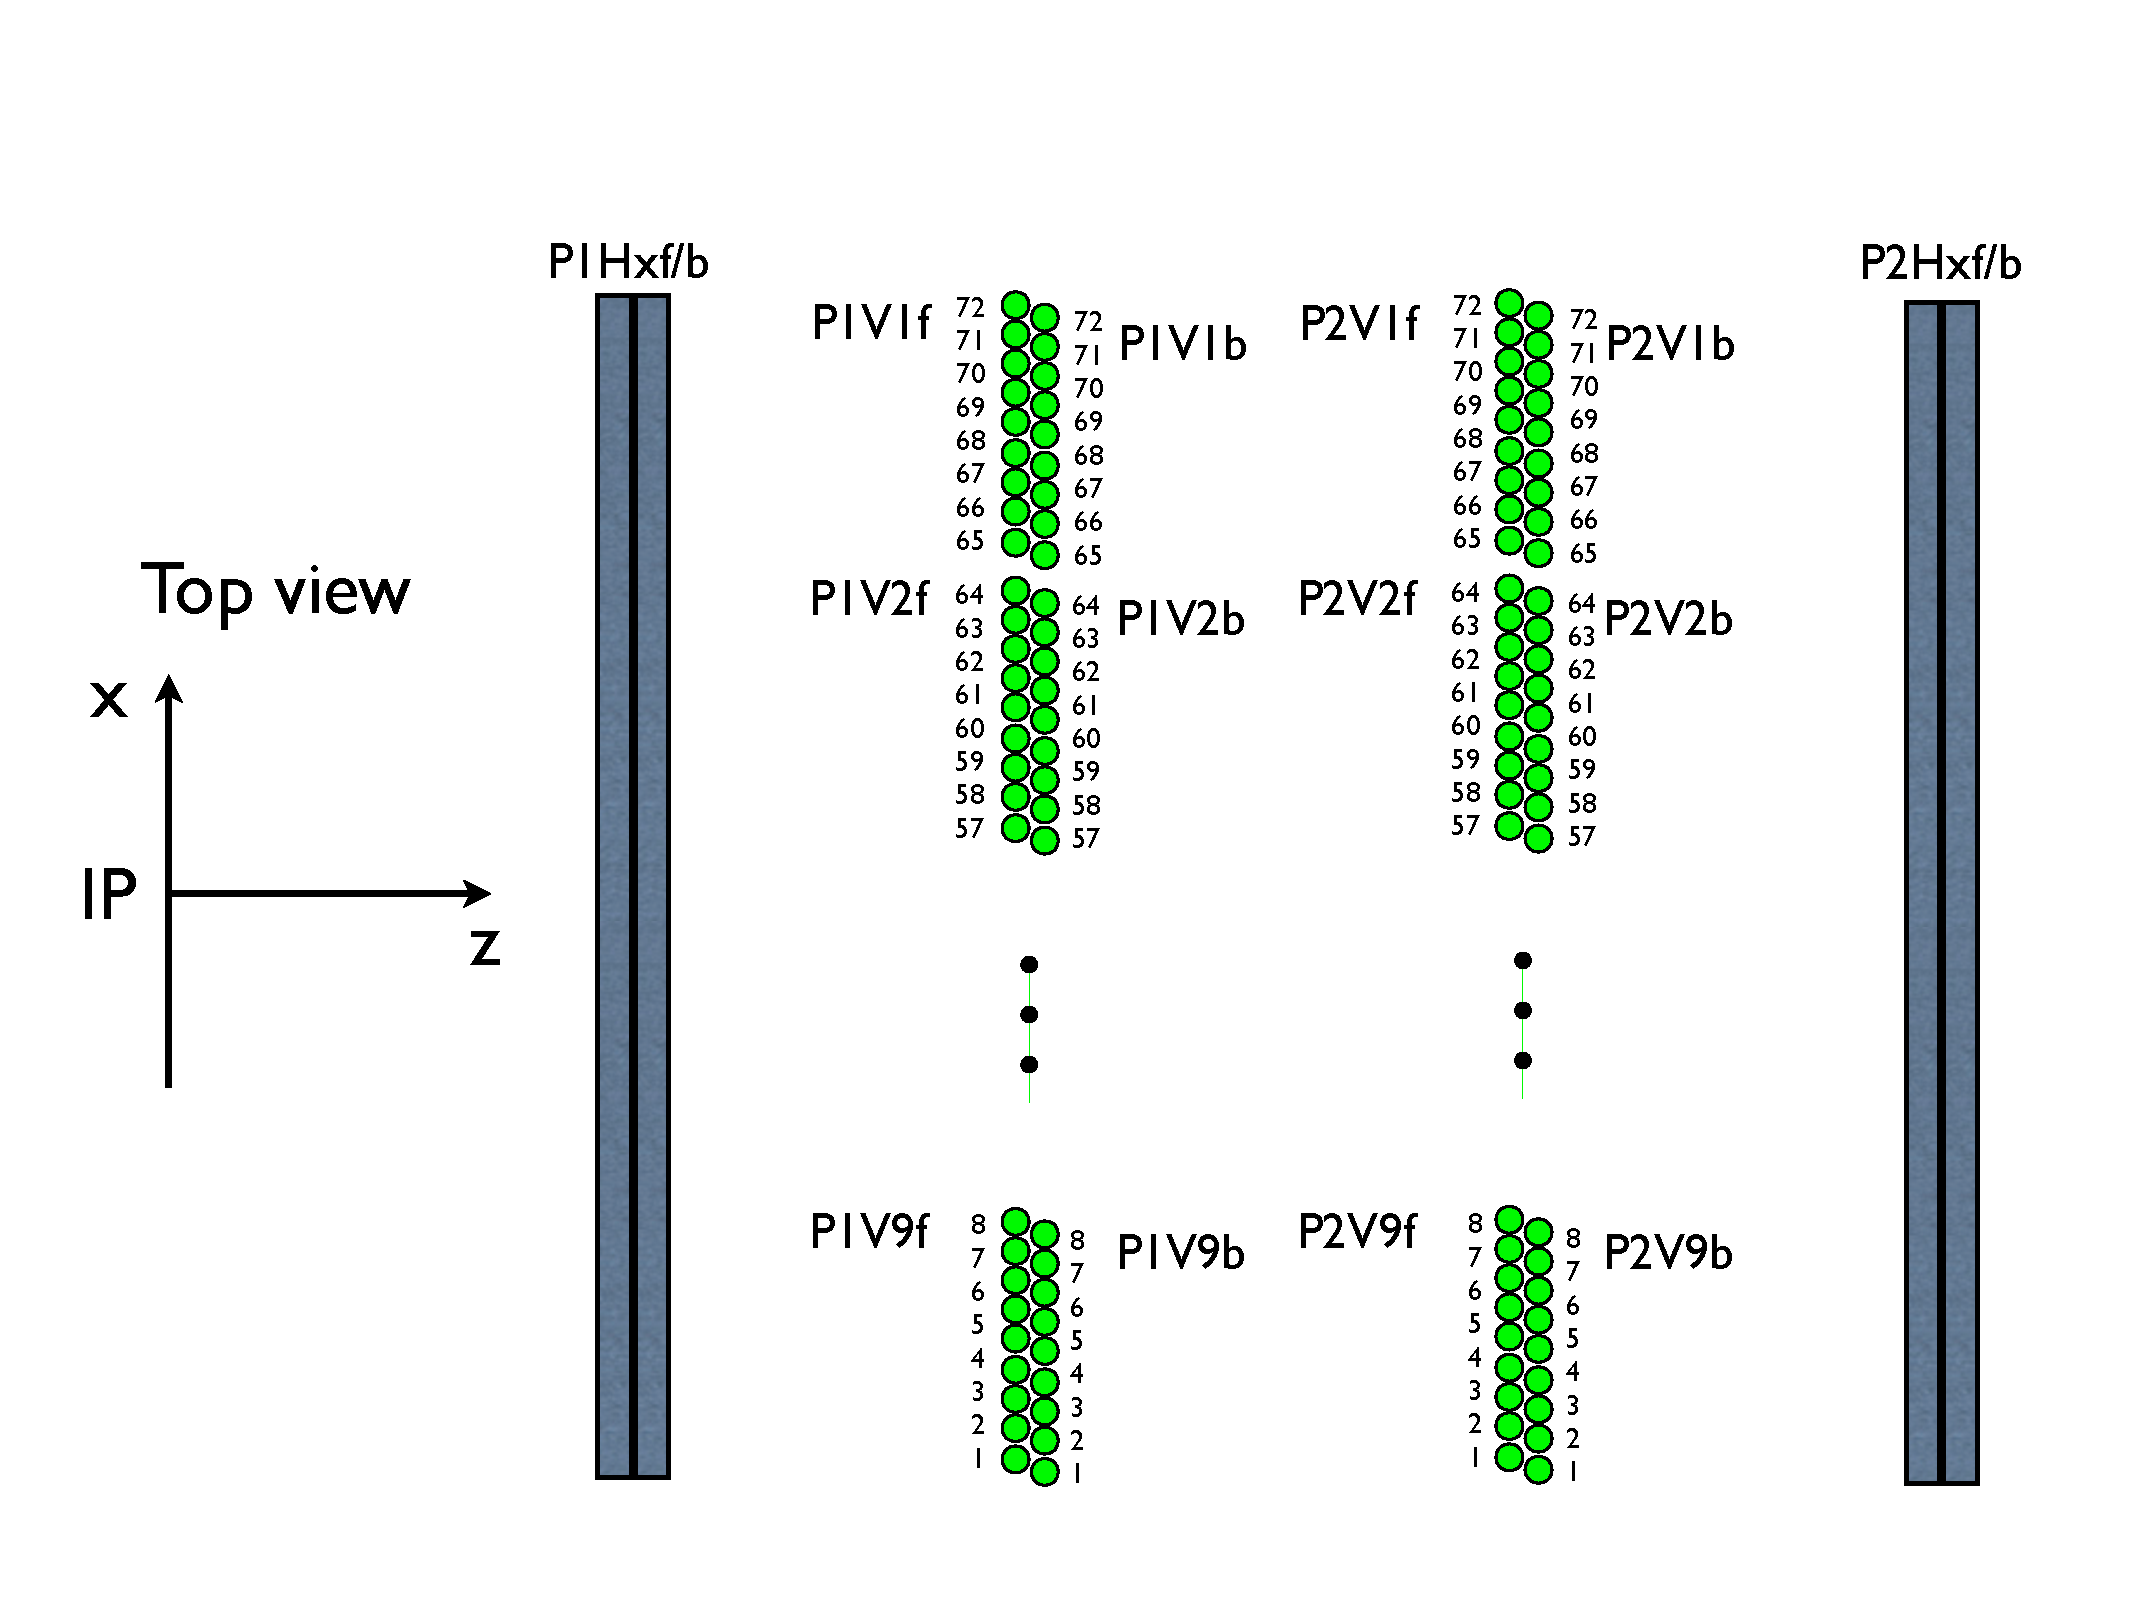
\includegraphics[width=\linewidth]{figures/proptubeview_xz.pdf}
		\caption{Proportional tube top ($x-z$ plane) view.}
		\label{fig:proptube:xzview}
	\end{minipage}
	\begin{minipage}[t]{0.49\linewidth}
		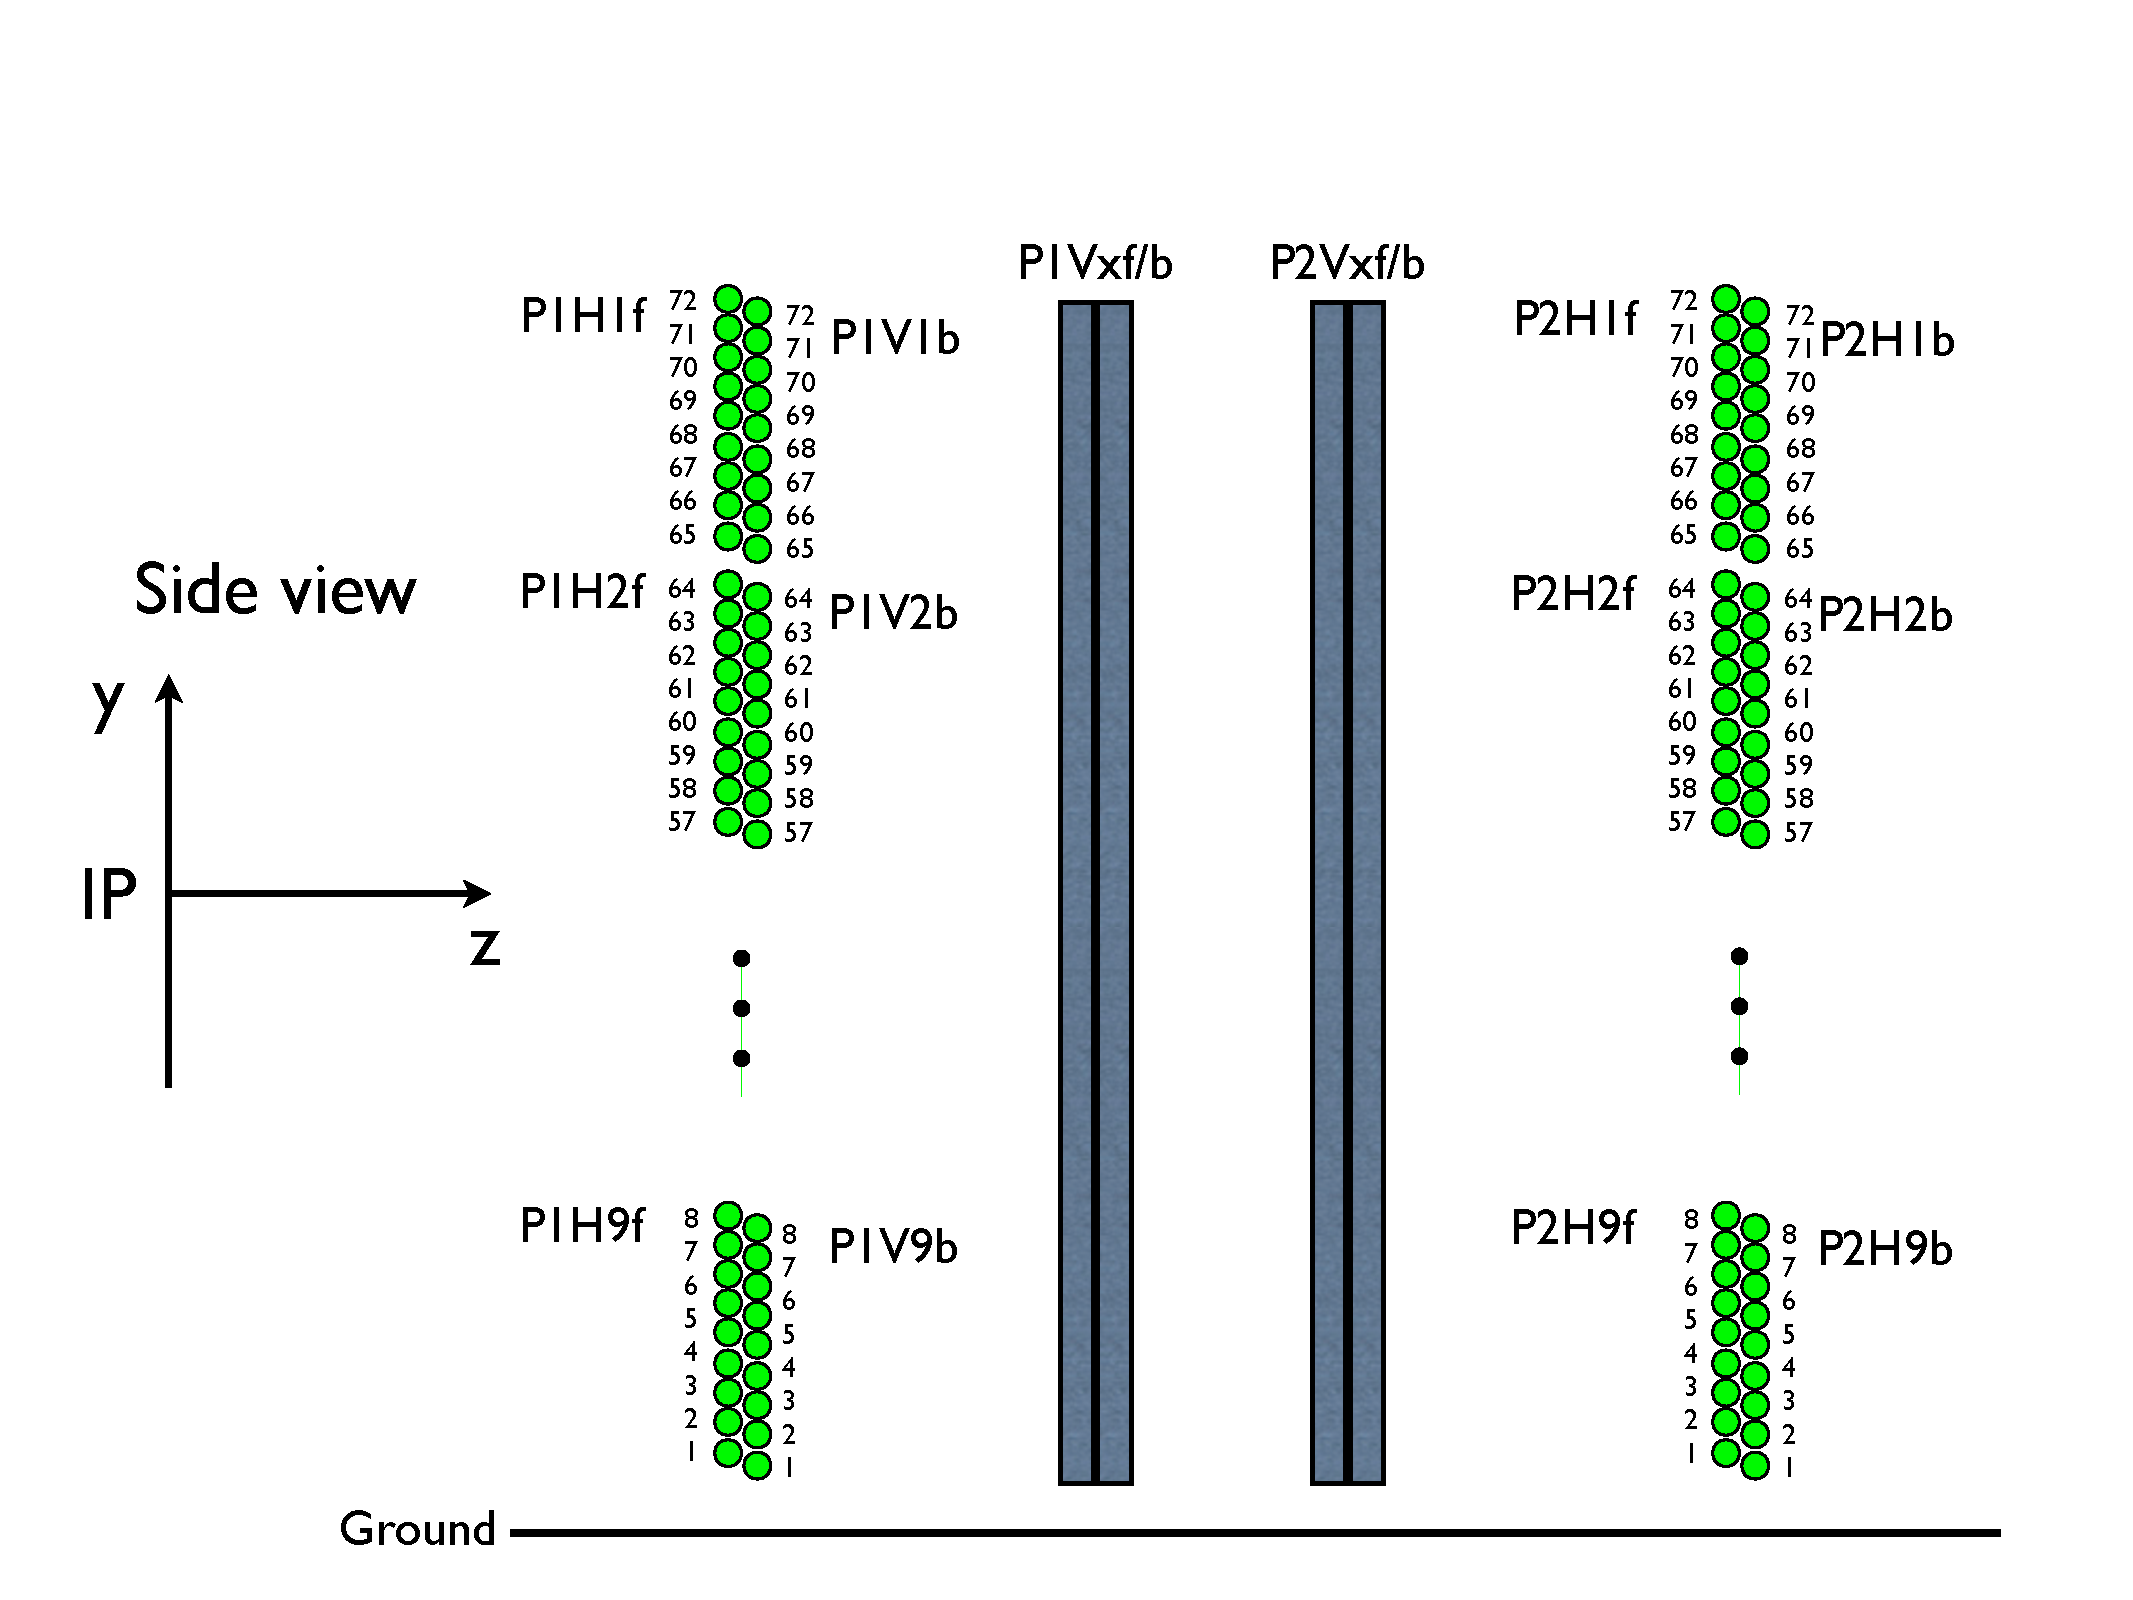
\includegraphics[width=1.03\linewidth]{figures/proptubeview_yz.pdf}
		\caption{Proportional tube side ($y-z$ plane) view.}
		\label{fig:proptube:yzview}
	\end{minipage}
\end{figure}

Each plane of proportional tubes is composed of 9 \emph{modules}, which each have a set of 16 proportional tubes: 8 in lined in an horizontal or vertical orientation and 8 more offset (``primed'') from the first 8 by 0.5 inches. This offset structure prevents any muons from going undetected between tubes and allows for left-right disambiguation for two hits in adjacent primed-unprimed sub-plane pairs in the same module. The modules are labeled $1-9$ in increasing order from left to right for the $x-$measuring planes and from $1-9$ in increasing order from top to bottom. So, the top module of the first vertical plane of prop tubes is P2H1. Additionally, in each module, the primed and unprimed sub-planes are referred to as \emph{f} for ``front'' (facing upstream) and \emph{b} for ``back'' (facing downstream). This substructure can be seen in detail on Fig.~\ref{fig:proptube:xzview} and Fig.~\ref{fig:proptube:yzview}.

A single prop tube is made of 2-inch diameter aluminum tubes with wall thickness of 1/16 inches. The central anode wire is a gold-plated $20 \mu$m diameter tungsten wire kept at approximately 1.95 kV. Considering the staggered nature of each plane's substructure, one can in principle achieve a spatial resolution of 0.3mm.  During Runs 2 and 3 of data taking, a resolution of 0.5mm for high energy muons was observed, which is more than sufficient for muon identification purpose. The gas mixture for prop-tubes is P-10 (Ar:Methane = 90:10) mixed with a $10\%$ CF4 gas (Ar:CO$_2$:CF$_4$ = 70:20:10) which yields the maximum drift time about 400ns. With this maximum, the prop tubes can handle a singles rate up to 2MHz, while normal operational hit rates are typically below 1MHz.

A typical desired high-energy muon within spectrometer acceptance will traverse through two prop-tubes in each plane and induces hit signals on two anode wires. The path of track is reconstructed from the drift time measured on the two anode output, with a custom TDC board that provides 0.44 ns timing resolution. With the hit information reconstructed from readouts of the forward and backward planes in $x-z$ and $y-z$ direction, precise reconstruction of the track trajectories can be obtained. Ideally, 8 hits from the 4 planes are used to form a track pointing back to the target. If such is the case, a candidate muon track is successfully identified.

\begin{table}[bthp]\centering
	\begin{tabular}{c|ccccc}
		\hline \hline
		Detector & Number   	& \# tubes 	& Width ($x$)           	& $z$-position \\
		Plane	 & of modules	& per	 	& $\times$ height ($y$)  	& of front (back)   \\ 
				 &    		    & module  	& [cm] $\times$ [cm]		& sub-plane	[cm]    \\ 
		\hline
		P1H    &  9     & 16  & 368 $\times$ 368 &  2,099 (+4)    \\
		P1V    &  9     & 16  & 368 $\times$ 368 &  2,175 (+4)    \\
		P2V    &  9     & 16  & 368 $\times$ 368 &  2,367 (+4)    \\
		P2H    &  9		& 16  & 368 $\times$ 368 &  2,389 (+4)    \\
		\hline
		\hline
	\end{tabular}
	\caption{Parameters of the four proportional tube planes.}
	\label{table:prop:param}
\end{table}

\subsection{Mass Resolution from Chamber Resolutions}

\begin{figure}
	\centering
	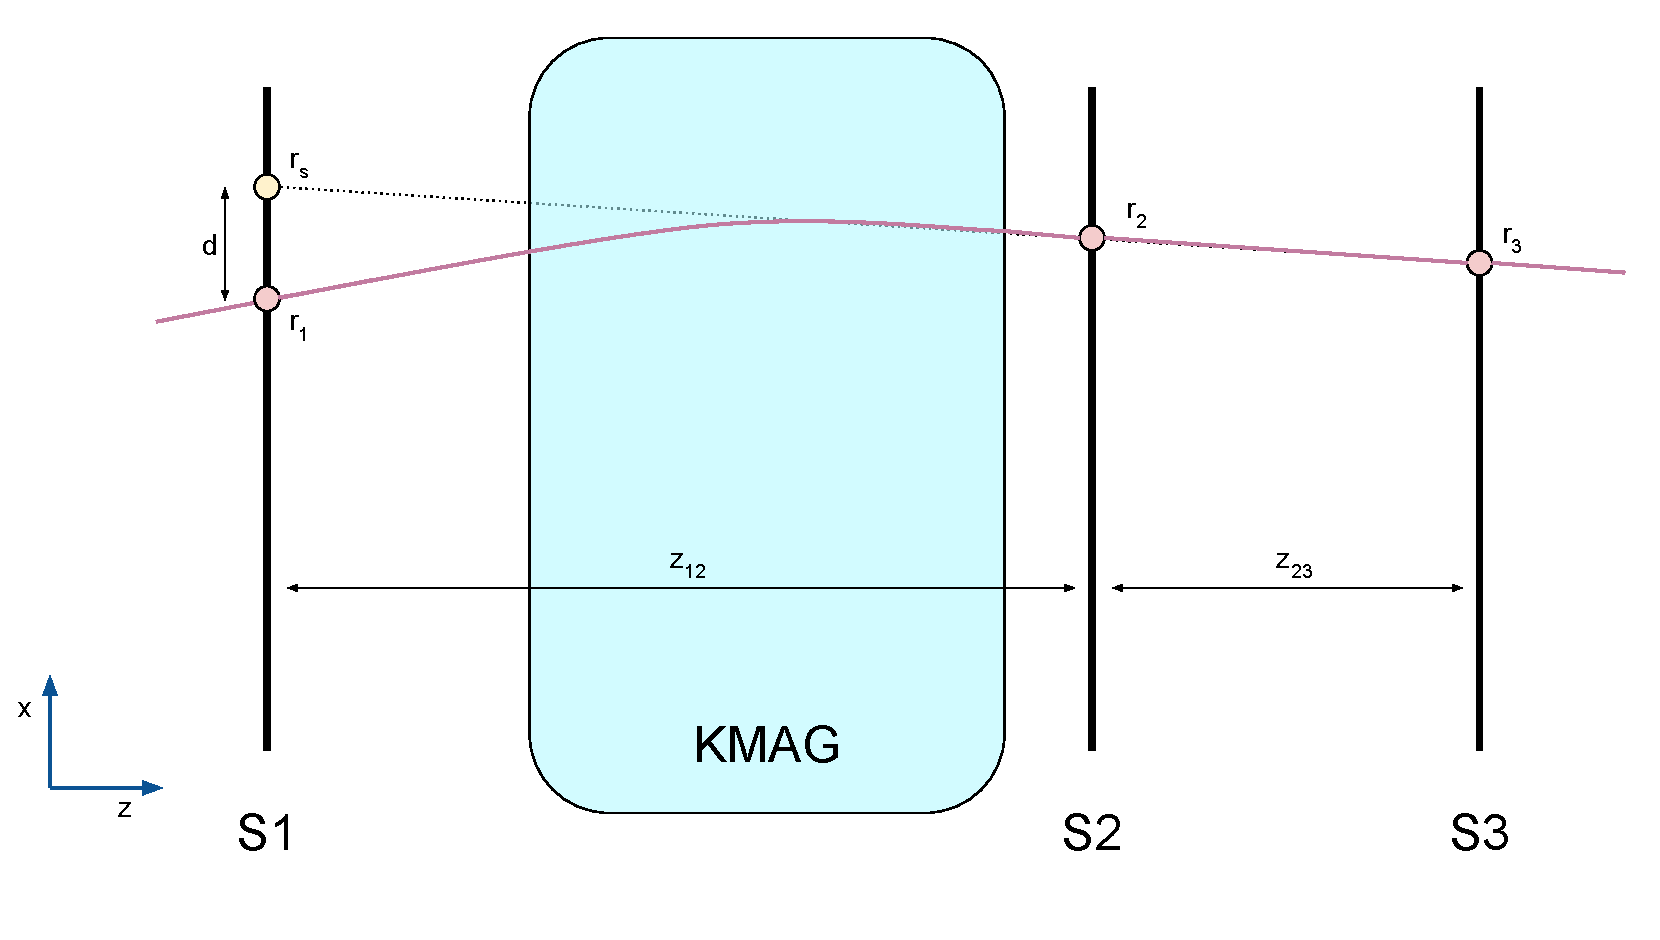
\includegraphics[width=0.75\textwidth]{figures/momentum-resolution.pdf}
	\caption{A simplistic depiction of a track passing through from Station 1, through KMAG where its path is bent by the magnetic field, and then straight on through Stations 2 and 3.}
	\label{fig:mom-res}
\end{figure}

The mass resolution of the spectrometer is, in part, limited by the resolution of the tracking chambers and the distances between them. For an arbitrary set of hit positions in Stations 1, 2, and 3 ($r_1, r_2, r_3$) which are separated from each other in $z$ by distances $z_{12}$ and $z_{23}$, with KMAG in between Stations 1 and 2 supplying a $P_{kick}$, one can derive $\Delta P / P$. A line, or track segment, is first reconstructed between $r_2$ and $r_3$. The slope (and its uncertainty) of this track segment in the $z-x$ plane is:
\begin{equation}
	s_{23} = \frac{r_3 - r_2}{z_{23}} \ \ ,\ \ \Delta s_{23} = \frac{1}{z_{23}}\sqrt{\Delta r_3^2 + \Delta r_2^2}
\end{equation}
The values of $\Delta r_n$ here are the position resolutions of the individual tracking chambers at each Station. One can use this slope to project a trajectory through KMAG and onto Station 1. The momentum is calculated by seeing where the actual hit position is in Station 1 and looking to the distance ($d$) between where the particle hit the station and where it would have hit had KMAG's magnetic field not existed. This is called a \emph{sagitta analysis}, as the magnetic field moves the particle's trajectory as if along a circle, and we are looking to the particle's path along the sagitta of that circle. Ultimately, the momentum uncertainty is related to this distance as:
\begin{equation}
	\frac{\Delta P }{P} = \frac{P}{P_{kick}}\Delta d
\end{equation}
The expected sagitta point ($r_s$) is located at:
\begin{eqnarray}
r_s & = & s_{23} z_{12} + r_2 \\
\Delta r_s = \sqrt{\Delta s_{23}^2 z_{12}^2 + \Delta r_2^2} & = & \sqrt{ \Delta r_3^2 \left(\frac{z_{12}}{z_{23}}\right)^2 + (1+\left(\frac{z_{12}}{z_{23}}\right)^2) \Delta r_2^2}
\end{eqnarray}
And the distance, $d$ follows as:
\begin{eqnarray}
d & = & r_s - r_1 \\
\Delta d = \sqrt{\Delta r_s^2 + \Delta r_1^2} & = & \sqrt{ \Delta r_3^2 \left(\frac{z_{12}}{z_{23}}\right)^2 + (1 + \left( \frac{z_{12}}{z_{23}} \right)^2) \Delta r_2^2 + \Delta r_1^2}
\end{eqnarray}
The momentum resolution due to chamber resolution can therefore be described as:
\begin{equation}
\frac{\Delta P}{P} = \frac{P}{P_{kick}} \sqrt{ \Delta r_3^2 \left(\frac{z_{12}}{z_{23}}\right)^2 + \left(1 + \left( \frac{z_{12}}{z_{23}} \right)^2 \right) \Delta r_2^2 + \Delta r_1^2}
\end{equation}
The dependence of the resolution on $P/P_{kick}$ works such that the larger the $P_{kick}$ is (w.r.t. particle momentum $P$), the more the track is bent, and the more precisely the original momentum is defined. Besides chamber resolution, other contributions to this momentum resolution are from multiple scattering through FMAG's iron beam dump and from the spectrometer's angular resolution. These will be discussed elsewhere in this paper.

The mass resolution is linked to momentum resolution via the following relation
\begin{equation}
\frac{\Delta M}{M} = \frac{\Delta P}{2 P}
\end{equation}
The factor of two arises from the fact that the Drell-Yan dilepton mass comes from two independent muons with the same momentum resolution. This mass resolution is important because it, in turn, contributes to the $\Delta x_2 / x_2$ resolution, which is the key dependent variable for SeaQuest measurements.
\begin{equation}
\frac{\Delta x_2}{x_2} \approx 0.57 \Delta x_F + 0.012 M^2 \frac{\Delta M}{M}
\end{equation}



\section{Trigger}

\begin{figure}
	\centering
	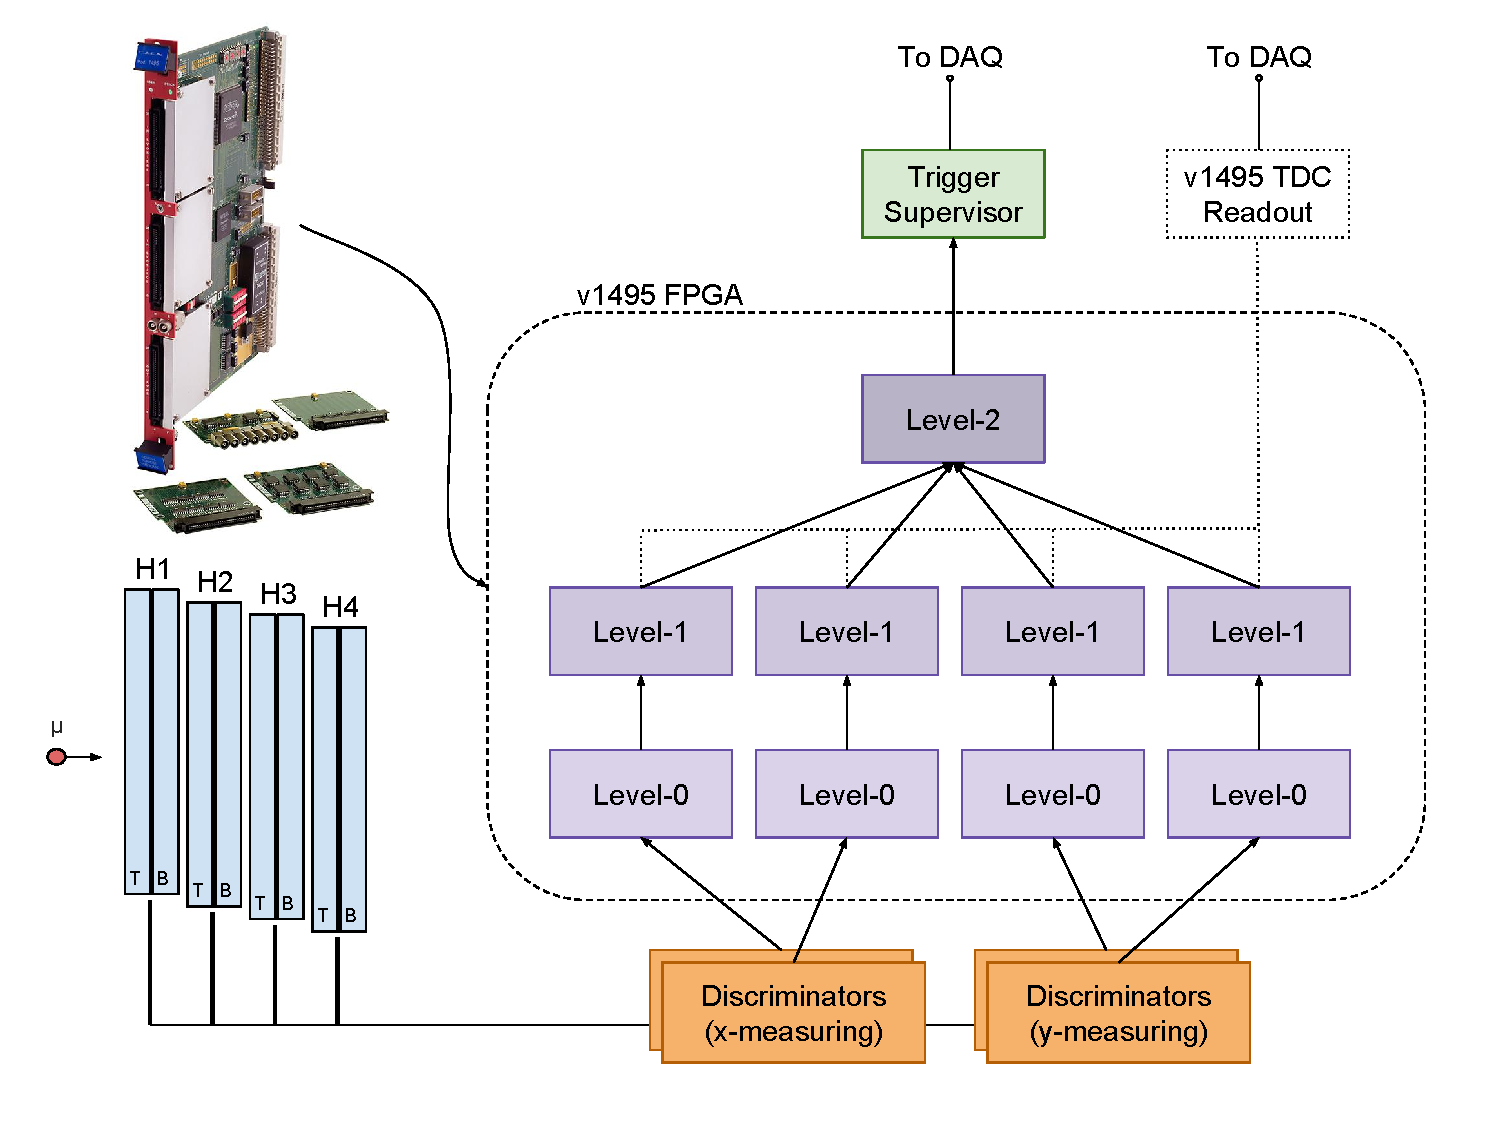
\includegraphics[width=0.75\textwidth]{figures/v1495-trigger.pdf}
	\caption{The trigger system at SeaQuest is composed of 9 CAEN v1495 FPGA modules. These modules output a trigger signal to the Trigger Supervisor, which tells the DAQ when to record data.}
	\label{fig:1495-trigger}
\end{figure}


The SeaQuest Trigger System selects candidate dimuon events from the high-rate environment using discriminated hodoscope signals. 

\subsection{Requirements}
%*select drellyan dimuons with acceptable efficiency*
The trigger must select events of interest to the main physics goals with high-enough efficiency to facilitate high-statistics analyses.
Therefore, the trigger is optimized to accept high-mass ($4-10$GeV) dimuons originating from the targets.
The trigger should intentionally reduce acceptance of dimuons from other, higher-rate sources, such as $J/\Psi$ decays and dimuons originating from the beam-dump.
The overall trigger rate must be kept low enough to maintain an acceptable DAQ livetime.
%*keep DAQ livetime high by minimizing trigger rate*
Additionally, the trigger should be internally deadtime-free. The trigger should be capable of firing on any and all RF-buckets while the DAQ is live.
%*internally deadtime free*
\par
The trigger should be sufficiently flexible to quickly accomodate changes in the spectrometer, beam conditions, and physics goals.
Any changes to the geometric acceptance of the spectrometer, whether caused by new/moved detectors, changes in the magnetic fields, or something else, must be immediately reflected in the trigger in order to maintain high-signal efficiency and high background rejection power.
Similarly, a change in the beam duty factor or intensity should be accompanied by a change in the trigger acceptance, ensuring trigger rate optimization.
Finally, the trigger should be capable of modifying the acceptance to facilitate special runs for other physics goals.
For these reasons, the design of the trigger system must allow for significant flexibility in the trigger-imposed acceptance.
%*flexibility*
\par
Lastly, the design of the trigger system should include self-diagnostic capabilities, allowing for constant monitoring of the trigger system's performance.
Internal pulser-testing is employed to test the function of each compiled firmware, every time the trigger logic changes.
Data from the internal TDCs is used by offline software to check the self-consistency of the trigger for each recorded physics event.
%*self-diagnostics (internal TDCs, internal pulser test)*


\begin{table}[bthp]\centering
  \caption{Performance of all DCs.
    That of DC1.2 is of anticipated values based on simulations,
    and those of the others are of measured values in Run 3.}
  \label{tab:cham:performance1}
  \begin{tabular}{c|ccc}
    \hline
    Trigger & Condition       & Sign    & \#$\mu$ \\
    \hline
    FPGA-1   &    T $\land$ B, 3-of-4    &   $+\land-$    &   2 \\
    FPGA-2   &    T $\lor$ B, 3-of-4      &  $+\lor-$       &  1 \\
    FPGA-3     &  T, 3-of-4       &    $+\lor-$   &   1  \\
    FPGA-4    &   B, 3-of-4       &    $+\lor-$    &   1 \\
    FPGA-5  &     T $\land$ B, 3-of-4       &     Any  &   2  \\
    NIM-1  &     T $\land$ B, 4-of-4       &     NA    &   NA   \\
    NIM-2  &     T $\land |$ B, X3-X4       &     NA    &   NA   \\
    \hline
  \end{tabular}
\end{table}

\section{Data Acquisition Systems}

\section{Data Productions}

\subsection{Production Processing}

The three raw outputs of the data acquisition systems, as described above are (1) Main DAQ CODA files, (2) Scaler DAQ CODA files, and (3) Beam DAQ ASCII files.

Each raw data file corresponds to the data taken from certain subsystems over approximately one to two hours of running time. These three types require varying degrees of de-serialization, parsing, processing, and storage -- a process as a whole defined as \emph{decoding}. 

All raw data files are backed up to long-term tape storage (managed by FNAL Computing Division), and the decoded and processed data gets stored on one of four MySQL servers to be used for analysis by the collaboration. Data is also output to a ROOT file for the ease of use of one of the two independent tracking programs.

Contiguous blocks of decoded and tracked data is then grouped together into \emph{merged} productions, available on all MySQL servers, providing collaborators large sets of curated and easily analyzable data.

\subsection{Decoding Raw Data}

The CODA file decoding is nearly identical for MainDAQ and ScalerDAQ, and only differ by content; the MainDAQ contains TDC readout. For each one to two hour \emph{Run}, the CODA files can be well-described as the following sequence of events (and the data they contain):
\begin{enumerate}
	\item Prestart Event (Run data)
	\item Begin Spill Event (Spill data, Scaler readout)
	\item Many Physics Events (Event data, TDC readout)
	\item End Spill Event (Spill data, Scaler readout)
	\item SlowControl Event (Slow control readout, Spill ID readout)
	\item Spill Counter Event (Spill ID readout) \newline ...(Repeat 2-6 for each \emph{Spill})
	\item End Event
\end{enumerate}

Our decoding program uses C and C++ in conjunction with Jefferson Lab's CODA I/O library to read these events and parse them according to their individual formats. Data from these CODA events are decoded and placed into hierarchical categories.

\subsubsection{Run Level Data}
Run-level data contains data and metadata pertaining to the entirety of the run that is recorded. At the time of the Prestart Event, the date and time of the run are stored, along with a readout of the specific settings of all non-trigger TDC boards.

After the End Event is encountered, metadata is aggregated and stored regarding such items as the number of chamber hits, the triggers that were fired, the target positions used, average magnet currents, and other useful metrics. 

\subsubsection{Spill Level Data}
The \emph{Beginning of Spill} (BOS) and \emph{End of Spill} (EOS) events bookend the set of physics events for a given spill. At each BOS and EOS events, the 140 MHz VME scalers are read out. At the beginning of the spill, all scalers should be zeroed out, and then read out again after the spill has ended.

Slow Control events are read out between spills, which contain data regarding the current spill identifier number, target systems, beam and radiation monitors, and environmental readings.

The spill identifier (\emph{spillID}) is what is used to synchronize the data together across various data acquisition systems. As such, the \emph{spillID} is read out redundantly in both Slow Control and Spill Counter events (which contain only the \emph{spillID} value) to ensure that the data is appropriately labeled.

When the End Event is reached, the independently-recorded Beam DAQ data (recorded in an ASCII file) is read and stored with the rest of the Spill-level data.

\subsubsection{Event Level Data}
For each spill, $\sim3k$ events are triggered to be recorded. With each event, three types of information is stored: the trigger which fired the event, a measure of the beam intensity per RF bucket, and the full detector readouts.
The detector readouts require the most processing of all the rest of the data. The CODA files contain the hardware addresses of each detector \emph{hit}, along with a \emph{TDC time}. The following steps briefly summarize the processing steps:
\begin{enumerate}
	\item Mapping: Map the hardware address to a detector name and detector element number
	\item Timing: Classify hits as in-time or not and calculate \emph{drift time} from TDC time
	\item R-T (time-to-space): Translate \emph{drift time} to \emph{drift distance}
	\item After-Pulse Elimination: Remove hits that result from signal reflection and other electronic artefacts
	\item Trigger Road Reconstruction: Use \emph{v1495} TDC hits to reconstruct possible trigger roads that may have fired
	\item Hodoscope Masking: Remove drift chamber hits that have no adjacent hodoscope hit
	\item Trigger Road Masking: Same as hodoscope masking, but only using hodoscopes from reconstructed trigger roads
\end{enumerate}
This fully processed data is then stored into one the experiment's MySQL databases.

%%%%%%%%%%%%%%%%

\subsection{Online and Offline Processing}

There are two modes of productions: on-line and off-line productions. For on-line productions, all Run- and Spill-level data is decoded, but only 1-in-$n$ Physics Events are processed, where $n$ is typically $15$. This \emph{``sampling mode''} is used in order for the decoding to reliably keep up with even high-intensity beam data.

For off-line productions, a large group of categorically similar runs is defined, and the chain of production processing is initiated. The steps of this process is generally emph{decoding, tracking, archiving, and merging}.

The decoding and tracking is performed on Fermilab Computing Service's FermiGrid, which provides the computing resources necessary to process hundreds of runs simultaneously.

A single decoding job submission will output the processed data to one of the four available MySQL servers and also to a ROOT file. Then, one job will be submitted to run one of the two tracking programs on the ROOT file, while another job is submitted to run the other tracking program on the MySQL data.

Once the tracking is completed, the ROOT file and the \emph{Hit} table from the MySQL production is archived on the Fermilab BlueArc NAS backup system for future use, if necessary.

Upon the completion of decoding and tracking of a specified range of runs, all of their Run-, Spill-, and Event-level data, along with its tracked data, is combined into a single \emph{merged} schema. These \emph{merged} schemas are mirrored across all four of the MySQL servers for optimal redundancy and availability.

\section{RDBMS Data Structure}

The processed data is primarily stored in MySQL Server 5.1 databases. MySQL is an open-source \textbf{R}elational \textbf{D}ata\textbf{b}ase \textbf{M}anagement \textbf{S}ystem (RDBMS) developed by Oracle that is well-suited for the storage and responsive querying of hierarchical data.

Each run is decoded into its own schema, and contains its own instances of all tables of a specified design. The tables are all \emph{join}-able to each other by sharing \emph{foreign keys} with each other in the form of the \emph{runID}'s, \emph{spillID}'s, and \emph{eventID}'s. The contents of the tables are \emph{indexed} in such a way that \emph{joins} and queries gain a speed performance boost, but this comes at the cost of disk space.

The data on the server is world-wide accessible and can be queried using the standard querying language. The queried data can be directed to any analysis code in any programming language due to the large array of MySQL API's available.

\section{Data Quality}

